\section{Onion Routing}
\label{onionrouting}
Onion routing is used to ensure sender-receiver anonymity. In contrast
to the Tor-network, there are no exit nodes and the receiver can be anyone
in the onion chain (see fig. \ref{onionrouting}).

\subsection{Variable Peers}
Different routes for every packet

\subsection{Source based routing}
Either here or in Intra Machine Intra Client
\subsection{Peer selection}
Which peers, how many. Constant? May give upper bounds of latency.

8 * 0.5seconds = 4 seconds delay.


%% \begin{figure}
%%     \centering
%%     \caption{Onion Routing}
%%     \label{onionrouting}
%%     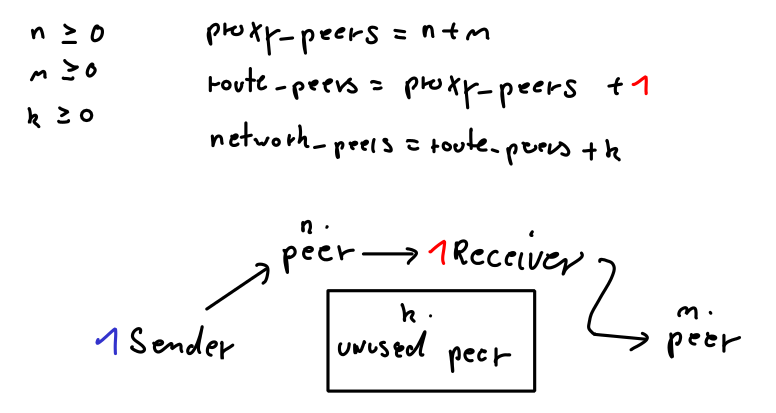
\includegraphics[scale=0.8]{onionrouting.eps}
%% \end{figure}
% ----------------------------------------------------------------------------
\subsection{Packet sizes}
The average packet size depending on the number of peers it was
(re-)encrypted for can be found in table \ref{pkgsizes}.
It was generated by running the reference implementation
(\verb=ceof onion -m "test" peer0  | wc -c=)
and increasing the number of proxy peers to be inserted.
The resulting size includes only the final onion,
but does not include transport protocol headers.
\begin{longtable}{|c|c|}
\caption{Packet sizes (experimental)}
\label{pkgsizes}\\
\hline
\textbf{Proxy peers} & \textbf{Packet size (in KiBiBytes)}\\
\hline
\textbf{1} & 1.2\\
\hline
\textbf{2} & 1.9\\
\hline
\textbf{3} & 2.6\\
\hline
\textbf{4} & 3.3\\
\hline
\textbf{5} & 4.0\\
\hline
\textbf{6} & 4.8\\
\hline
\textbf{7} & 5.6\\
\hline
\textbf{8} & 6.3\\
\hline
\textbf{9} & 7.1\\
\hline
\textbf{10} & 8.0\\
\hline
\end{longtable}



